\subsection{Fits\-Image  Class Reference}
\label{class_fitsimage}\index{FitsImage@{Fits\-Image}}
This class enables basic manipulation of images stored in fits files. 


{\tt \#include $<$fitsimage.h$>$}

Inheritance diagram for Fits\-Image::\begin{figure}[H]
\begin{center}
\leavevmode
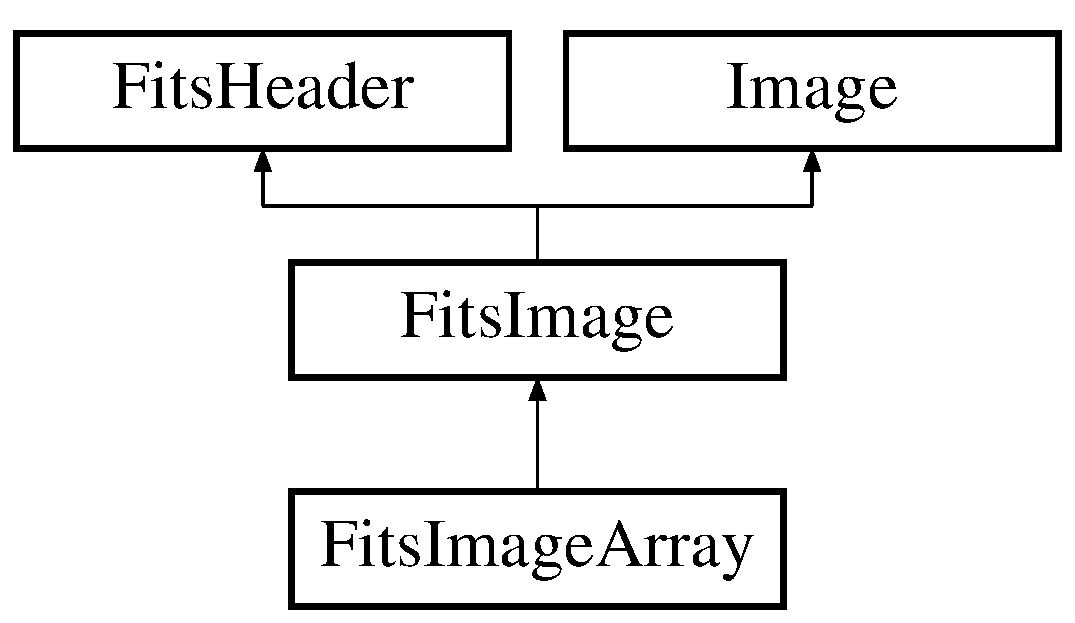
\includegraphics[height=3cm]{class_fitsimage}
\end{center}
\end{figure}
\subsubsection*{Public Methods}
\begin{CompactItemize}
\item 
\index{FitsImage@{FitsImage}!FitsImage@{Fits\-Image}}\index{FitsImage@{FitsImage}!FitsImage@{Fits\-Image}}
{\bf Fits\-Image} (const string \&File\-Name, const Fits\-File\-Mode Mode=RO)\label{class_fitsimage_a0}

\begin{CompactList}\small\item\em opens in (Read\-Only mode by default, use RW to modifiy or create) and loads the pixel data.\item\end{CompactList}\item 
\index{FitsImage@{FitsImage}!FitsImage@{Fits\-Image}}\index{FitsImage@{FitsImage}!FitsImage@{Fits\-Image}}
{\bf Fits\-Image} (const {\bf Fits\-Header} \&Header)\label{class_fitsimage_a1}

\begin{CompactList}\small\item\em constructor to be used starting from an existing {\bf Fits\-Header} {\rm (p.\,\pageref{class_fitsheader})}.\item\end{CompactList}\item 
{\bf Fits\-Image} (const string \&New\-File\-Name, const {\bf Fits\-Header} \&a\_\-fits\_\-header, const {\bf Image} \&an\_\-image)
\begin{CompactList}\small\item\em constructor for a new Fits\-Image.\item\end{CompactList}\item 
\index{FitsImage@{FitsImage}!FitsImage@{Fits\-Image}}\index{FitsImage@{FitsImage}!FitsImage@{Fits\-Image}}
{\bf Fits\-Image} (const string \&New\-File\-Name, const {\bf Fits\-Header} \&AHeader)\label{class_fitsimage_a3}

\begin{CompactList}\small\item\em constructor of a new Fits\-Image using an existing header, a new name, and a zeroed {\bf Image} {\rm (p.\,\pageref{class_image})}. RW mode.\item\end{CompactList}\item 
\index{FitsImage@{FitsImage}!FitsImage@{Fits\-Image}}\index{FitsImage@{FitsImage}!FitsImage@{Fits\-Image}}
{\bf Fits\-Image} (const string \&File\-Name, const {\bf Image} \&an\_\-image)\label{class_fitsimage_a4}

\begin{CompactList}\small\item\em constructor for a new Fits\-Image with a minimal header from an existing image.\item\end{CompactList}\item 
\index{FitsImage@{FitsImage}!FitsImage@{Fits\-Image}}\index{FitsImage@{FitsImage}!FitsImage@{Fits\-Image}}
{\bf Fits\-Image} (const string \&File\-Name, const int Nx, const int Ny)\label{class_fitsimage_a5}

\begin{CompactList}\small\item\em constructor for a new Fits\-Image with a minimal header from scratch.\item\end{CompactList}\item 
\index{Trim@{Trim}!FitsImage@{Fits\-Image}}\index{FitsImage@{FitsImage}!Trim@{Trim}}
void {\bf Trim} (const {\bf Frame} \&Region)\label{class_fitsimage_a6}

\begin{CompactList}\small\item\em Extract and replaces the trimed {\bf Image} {\rm (p.\,\pageref{class_image})} into a Fits\-Image.\item\end{CompactList}\item 
\index{PreserveZeros@{PreserveZeros}!FitsImage@{Fits\-Image}}\index{FitsImage@{FitsImage}!PreserveZeros@{Preserve\-Zeros}}
void {\bf Preserve\-Zeros} ()\label{class_fitsimage_a7}

\begin{CompactList}\small\item\em This routine is to be called if one wants to preserve the value of 0 on I/O. Assumes contents $>$=0, as it is Used for weight maps.\item\end{CompactList}\item 
\index{~FitsImage@{$\sim$FitsImage}!FitsImage@{Fits\-Image}}\index{FitsImage@{FitsImage}!~FitsImage@{$\sim$Fits\-Image}}
{\bf $\sim$Fits\-Image} ()\label{class_fitsimage_a8}

\item 
\index{SetWriteAsFloat@{SetWriteAsFloat}!FitsImage@{Fits\-Image}}\index{FitsImage@{FitsImage}!SetWriteAsFloat@{Set\-Write\-As\-Float}}
bool {\bf Set\-Write\-As\-Float} ()\label{class_fitsimage_a9}

\item 
\index{Write@{Write}!FitsImage@{Fits\-Image}}\index{FitsImage@{FitsImage}!Write@{Write}}
int {\bf Write} (bool force\_\-bscale=false)\label{class_fitsimage_a10}

\item 
\index{Write@{Write}!FitsImage@{Fits\-Image}}\index{FitsImage@{FitsImage}!Write@{Write}}
int {\bf Write} (const double \&Bscale, const double \&Bzero)\label{class_fitsimage_a11}

\end{CompactItemize}


\subsubsection{Detailed Description}
This class enables basic manipulation of images stored in fits files.

For The image itself, see the {\bf Image} {\rm (p.\,\pageref{class_image})} class. The files opened in mode RW are actually written to disk by the destructor. {\bf Fits\-Header::Enable\-Write}() {\rm (p.\,\pageref{class_fitsheader_a45})} allows to alter this default behavior. 



\subsubsection{Constructor \& Destructor Documentation}
\index{FitsImage@{Fits\-Image}!FitsImage@{FitsImage}}
\index{FitsImage@{FitsImage}!FitsImage@{Fits\-Image}}
\paragraph{\setlength{\rightskip}{0pt plus 5cm}Fits\-Image::Fits\-Image (const string \& {\em New\-File\-Name}, const {\bf Fits\-Header} \& {\em a\_\-fits\_\-header}, const {\bf Image} \& {\em an\_\-image})}\hfill\label{class_fitsimage_a2}


constructor for a new Fits\-Image.

To be used to assemble a Fits\-Image from a header and an image obtained separately. The associated mode is RW. The actual size of the saved image is the one of the image, not the one in the header. 

The documentation for this class was generated from the following file:\begin{CompactItemize}
\item 
{\bf fitsimage.h}\end{CompactItemize}
